\section{\textit{FrontEnd}}
\label{chap:frontend}

Di seguito viene illustrata la parte \textit{FrontEnd} del progetto. 
\subsection{Autenticazione}
\begin{figure}[H]
    \centering
    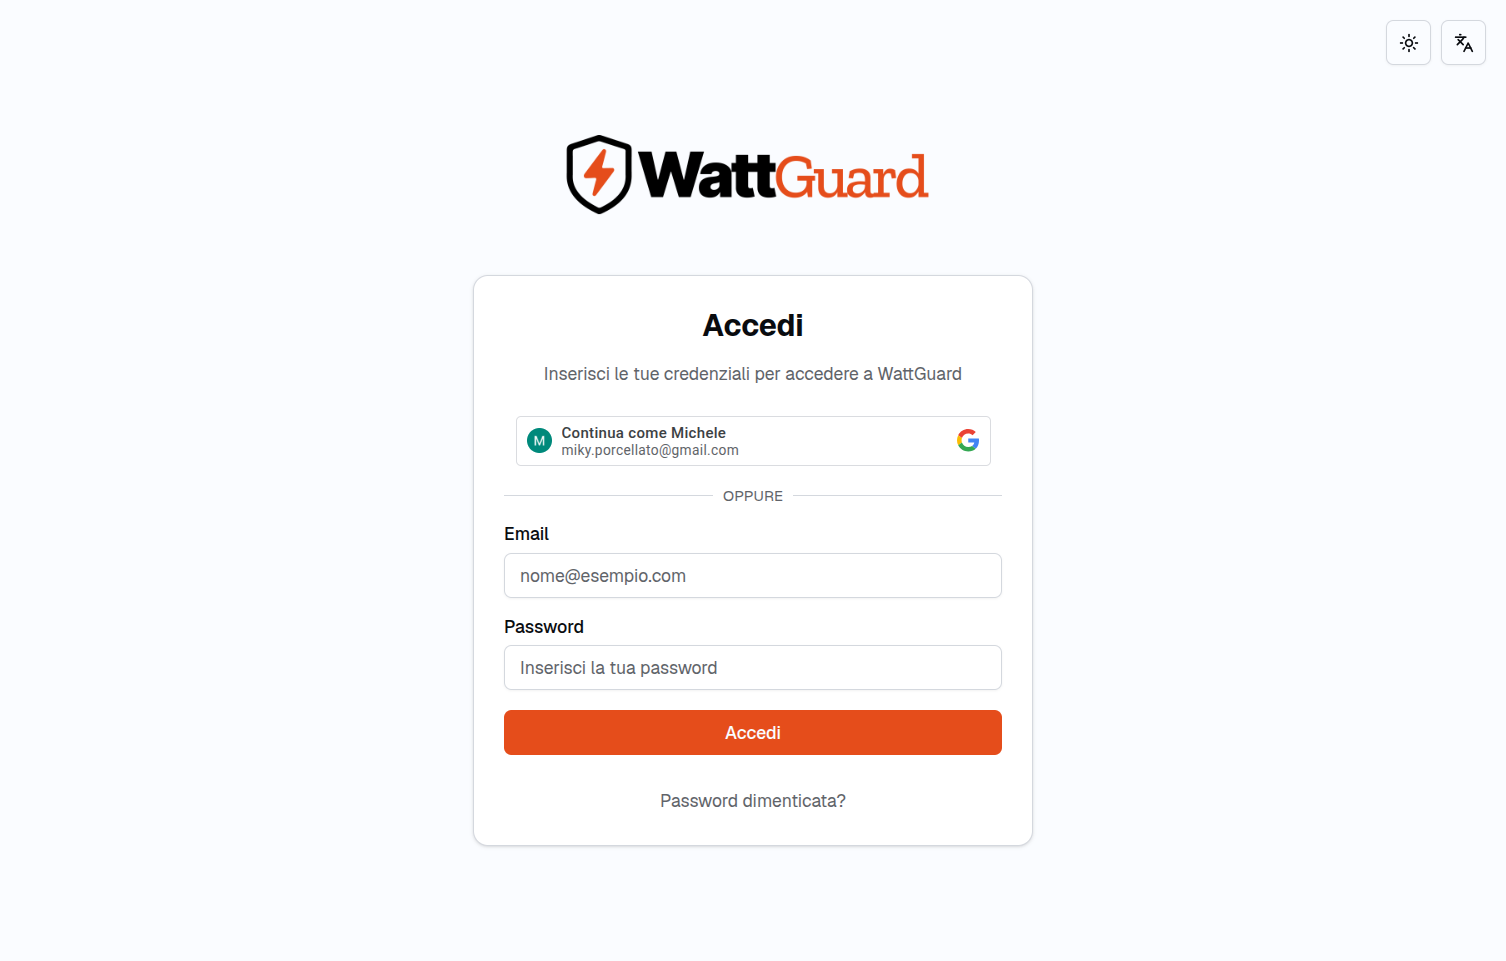
\includegraphics[width=0.75\linewidth]{../images/Frontend/login.png}
    \caption{Pagina di login}
    \label{fig:login}
\end{figure}

\begin{figure}[H]
    \centering
    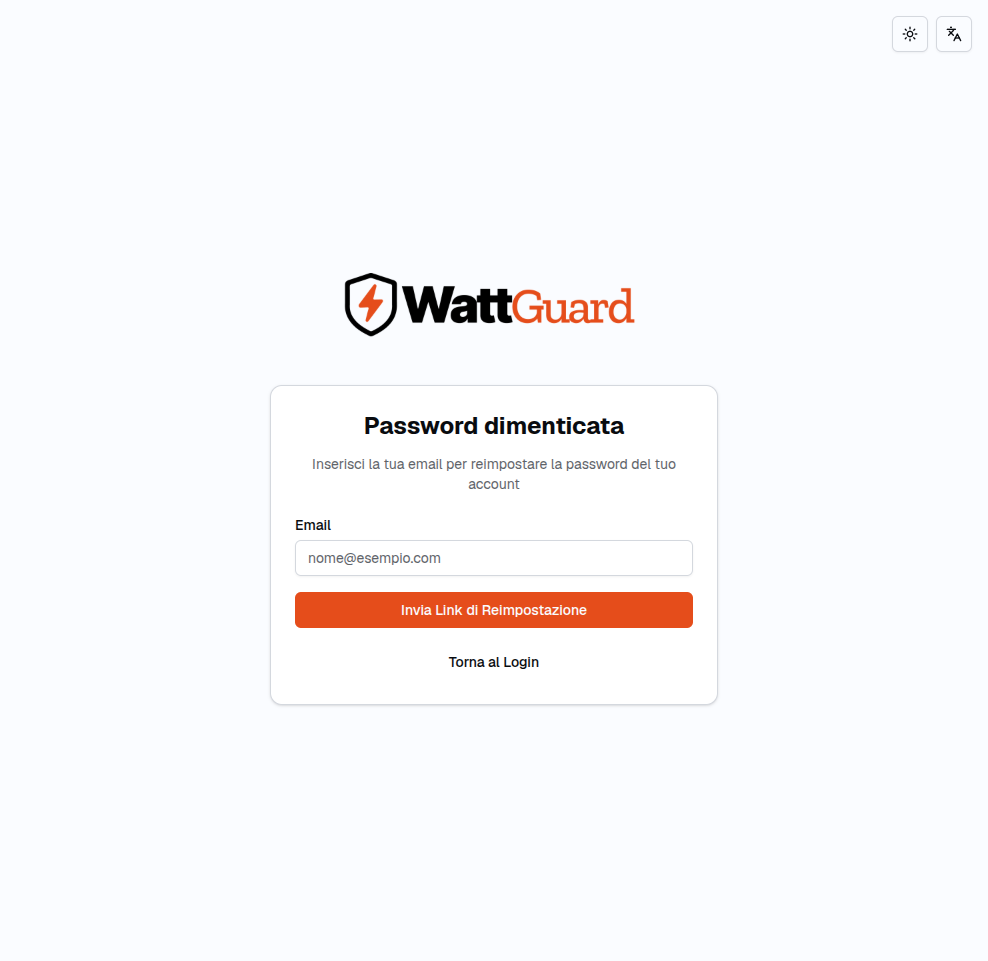
\includegraphics[width=0.5\linewidth]{../images/Frontend/forgot-password.png}
    \caption{Reset Password}
    \label{fig:reset-password}
\end{figure}


Nella \cref{fig:login} è presente la pagina principale di login, alla quale l'utente è condotto se non è attualmente loggato o il token di autenticazione JWT è scaduto.
È possibile autenticarsi sia tramite credenziali locali, inserendo e-mail e password, sia attraverso il pulsante ``Accedi con Google''

Durante la risoluzione dello stato di autenticazione viene mostrato uno \emph{spinner}.
Se l'utente viene autenticato con successo, viene reindirizzato alla dashboard principale.

Nella stessa sezione è possibile procedere con il recupero della password. (\cref{fig:reset-password})
\subsection{Accettazione Invito}

\begin{figure}[H]
    \centering
    % Prima immagine
    \begin{subfigure}[b]{0.48\textwidth}
        \centering
        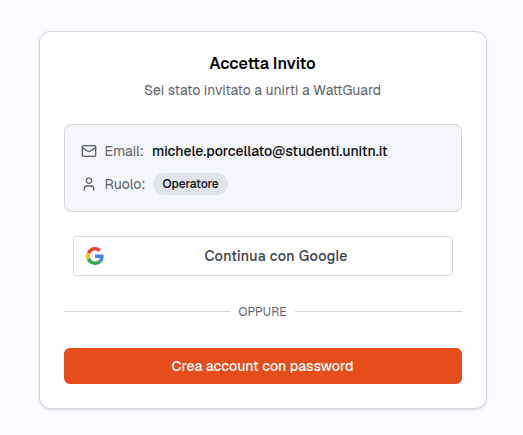
\includegraphics[width=\linewidth]{../images/Frontend/accept-invite-1.png}
        \label{fig:accept-invite-1}
    \end{subfigure}
    \hfill % Spazio orizzontale flessibile per separare le due figure
    % Seconda immagine
    \begin{subfigure}[b]{0.48\textwidth}
        \centering
        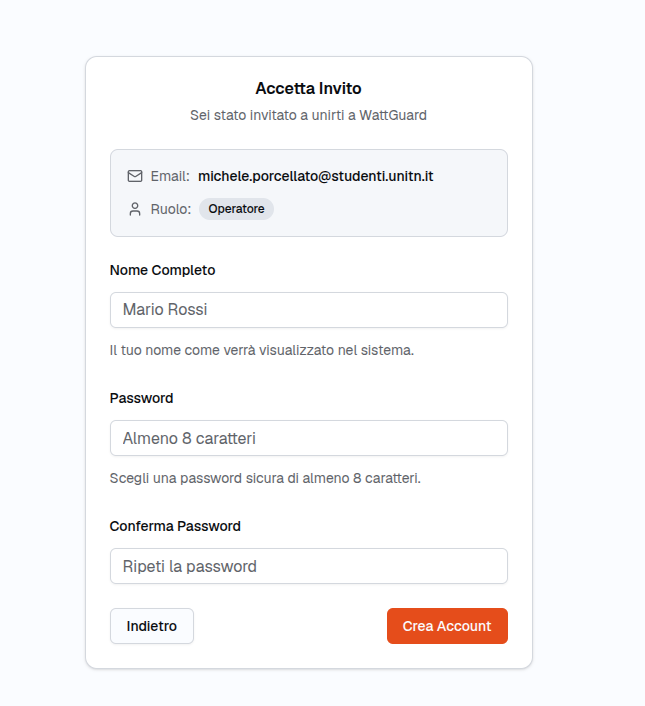
\includegraphics[width=\linewidth]{../images/Frontend/accept-invite-2.png}
        \label{fig:accept-invite-2}
    \end{subfigure}
    
    \caption{Flow di accettazione invito}
    \label{fig:accept-invite}
\end{figure}

Come illustrato nella \cref{fig:accept-invite} si illustano i passaggi necessari per accettare l'invito e completare la registrazione. Durante la registrazione è possibile procedere con il login con Google oppure creare manualmente l'utente.
Se si decide di procedere con la creazione manuale, è richiesto compilare il modulo con nome utente e password.

\subsection{Layout della dashboard}

\begin{figure}[H]
    \centering
    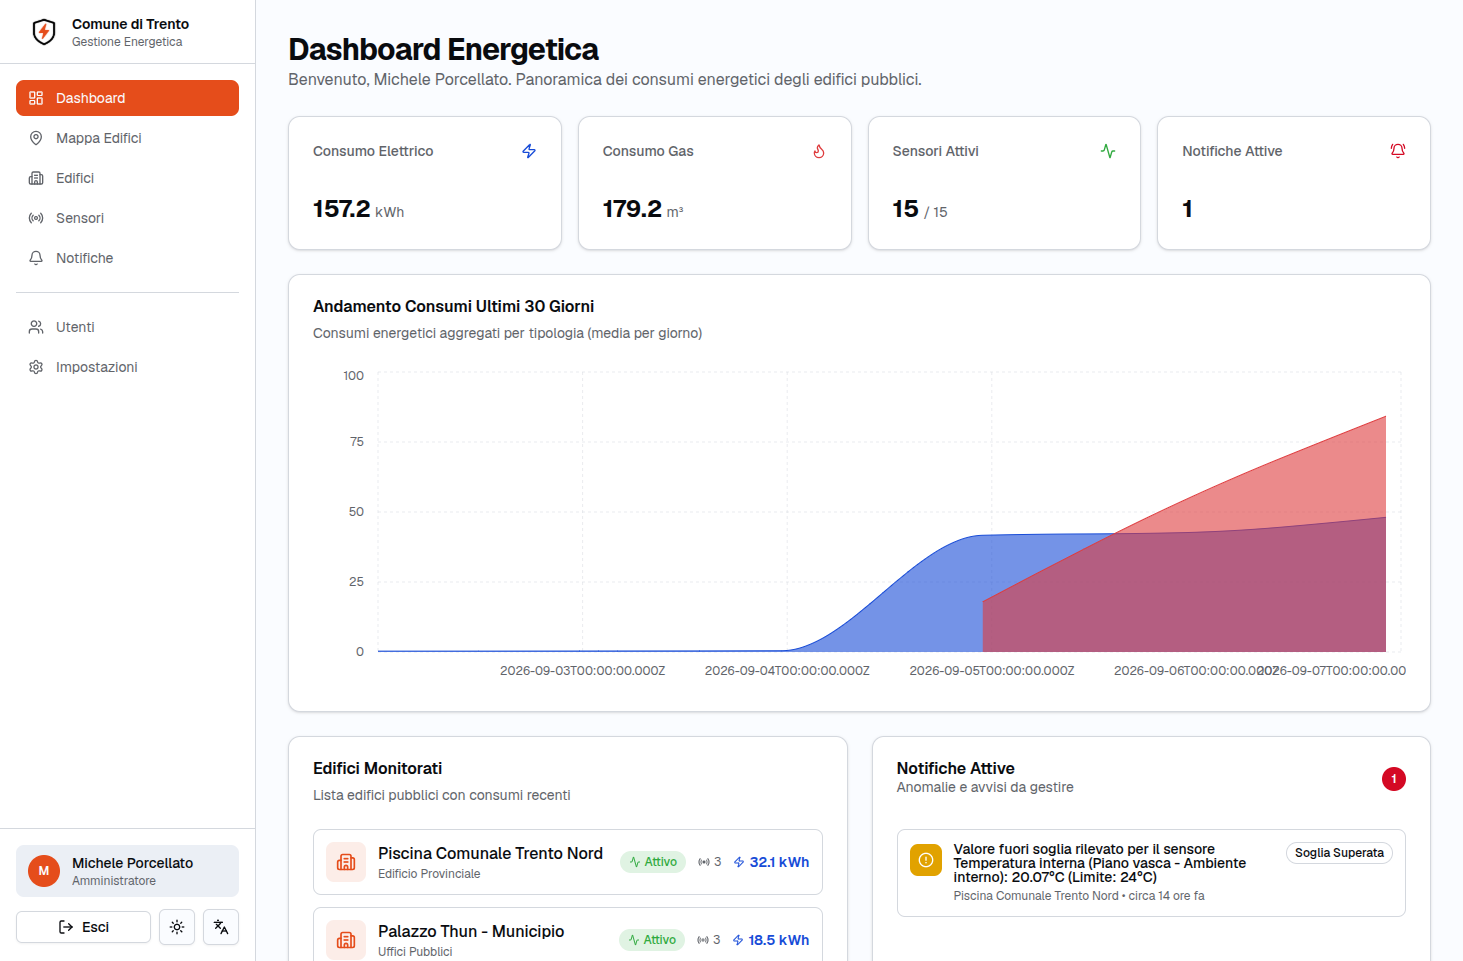
\includegraphics[width=0.80\linewidth]{../images/Frontend/dashboard.png}
    \caption{Dashboard pricnipale}
    \label{fig:dashboard}
\end{figure}

Dopo l'autenticazione l'utente si trova all'interno della dashboard. (\cref{fig:dashboard}).

Osserviamo la presenza della nav-bar a lato, la quale indica che pagina è attualmente selezionata (dashboard generare, mappa degli edifici, ricerca edifici, sensori e notifiche) e informazioni sull'utente attualmente loggato. In basso si trova il pulsante per eseguire il logout, il selettore per cambiare il tema predefinito e il selettore per cambiare la lingua del frontend (it/en/de).
Le sezioni di utenti e impostazioni sono presenti soltato per 
gli amministratori.
\newline\newline
La pagina della dashboard principale contiene i seguenti componenti:
\begin{itemize}
    \item \textbf{Informazioni complessive del sistema}: Questa sezione contiene il consumo elettrico complessivo attuale, il consumo di gas degli ultimi 30 giorni, il sensori attivi (non in manutenzione o offline) e le notifiche presenti.
    \item  \textbf{Grafico andamento dei consumi}: Il grafico mostra i consumi energetici aggregati per tipologia (celeste il consumo elettrico mentre il gas in rosso) degli ultimi 30 giorni.
    Facendo hover sul grafico compare un tooltip che mostra i dettagli del singolo punto selezionato.
    \item \textbf{Edifici Monitorati}: Mostra la lista degli edifici con i loro consumi recenti. È presente inoltre l'indicatore di quanti sensori sono presenti nell'edifico, se l'edificio è attivo o dismesso e il loro consumo istantaneo di corrente elettrica.
    \item \textbf{Notifiche attive}: Questa sezione serve per ricordare agli amministratori e agli operatori di eventuali anomalie presenti negli edifici monitorati.
\end{itemize}

I dati presenti nella dashboard vengono aggiornati automaticamente ogni 90 secondi. Questo intervallo è configurabile all'interno delle impostazioni di sistema.

\subsection{Mappa degli edifici}

\begin{figure}[H]
    \centering
    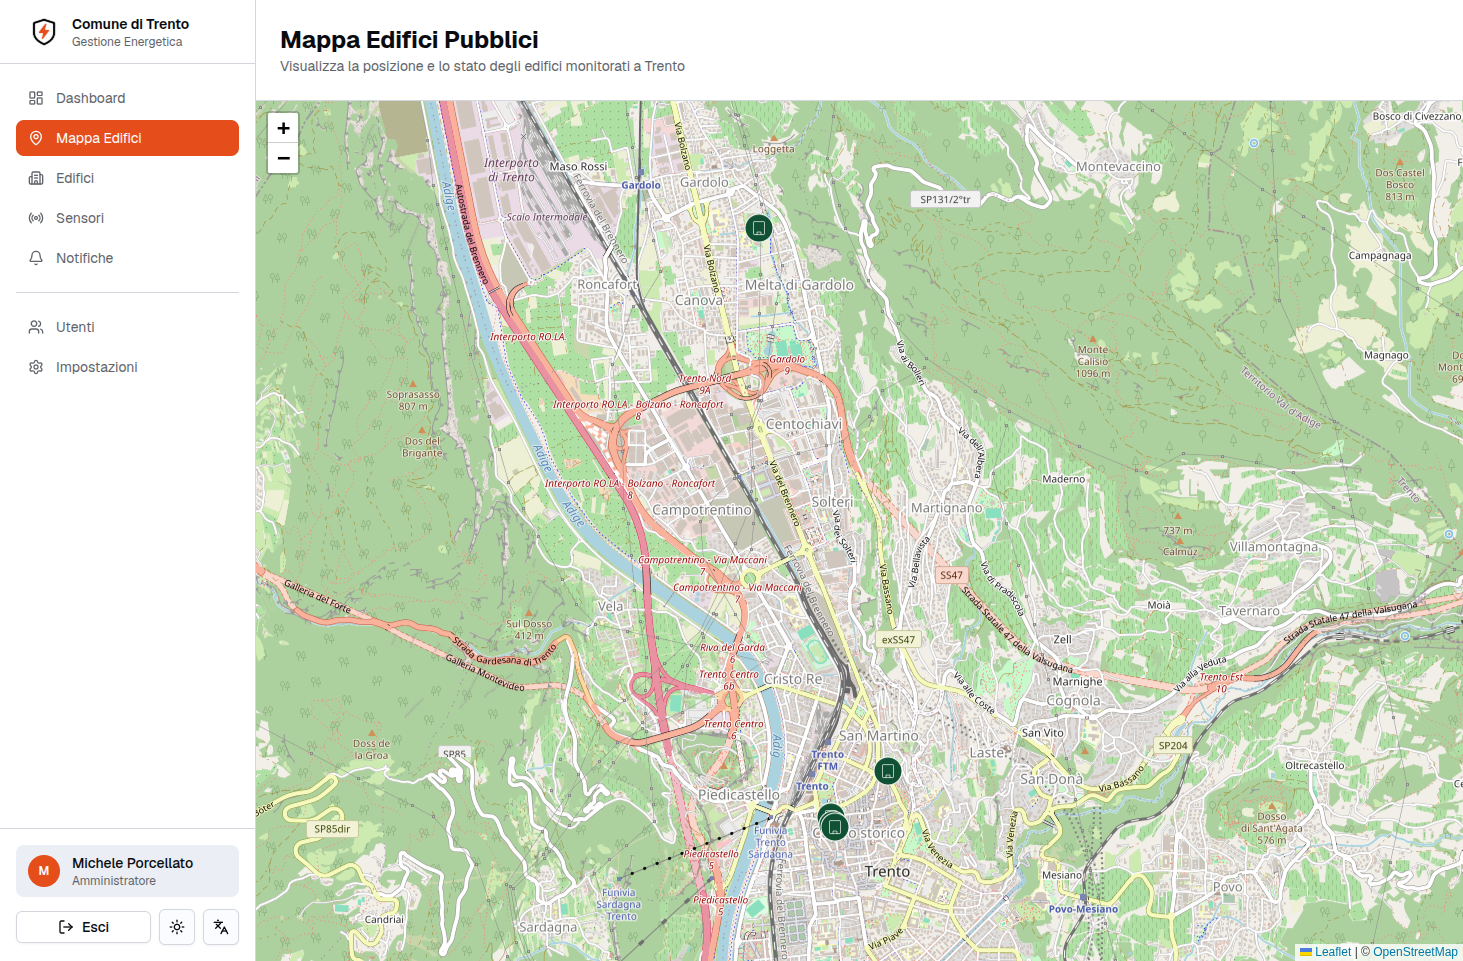
\includegraphics[width=0.80\linewidth]{../images/Frontend/map.png}
    \caption{Mappa edifici}
    \label{fig:map}
\end{figure}

Nella \cref{fig:map} si mostra la pagina contenete la disposizione geografica degli edifici monitorati su una mappa interattiva. Ogni edificio è rappresentato da un marcatore; selezionandolo, l'utente accede al dettaglio dell'edificio.
Il marcatore è verde se l'edifico risulta attivo, grigio se dismesso.

\subsection{Edifici}

\begin{figure}[H]
    \centering
    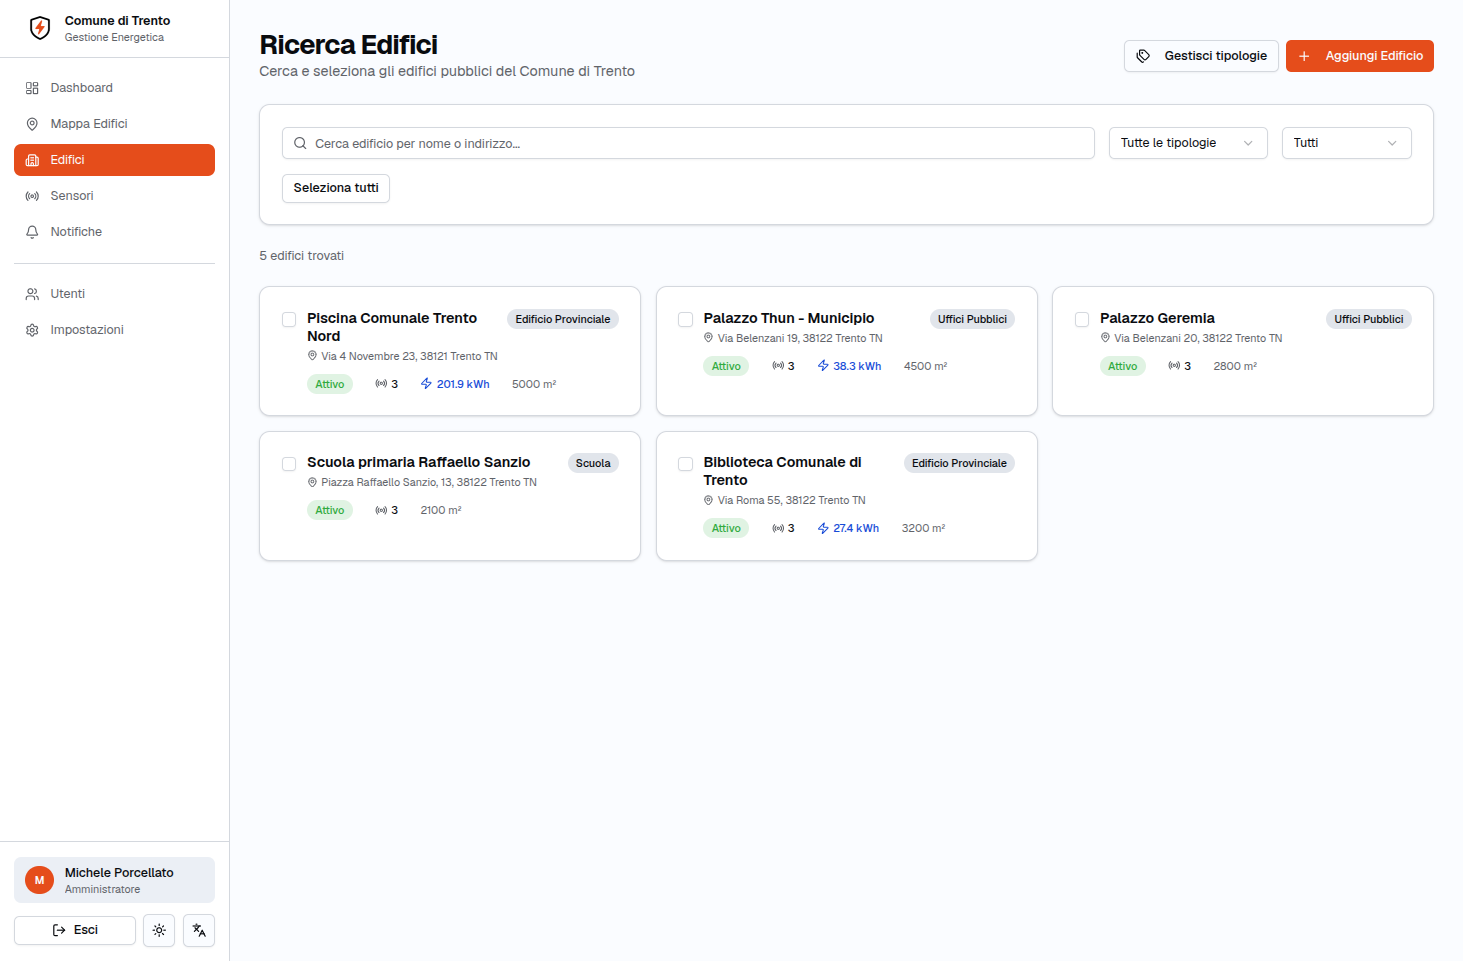
\includegraphics[width=0.80\linewidth]{../images/Frontend/buildings.png}
    \caption{Elenco edifici con ricerca}
    \label{fig:buildings}
\end{figure}

\begin{figure}[H]
    \centering
    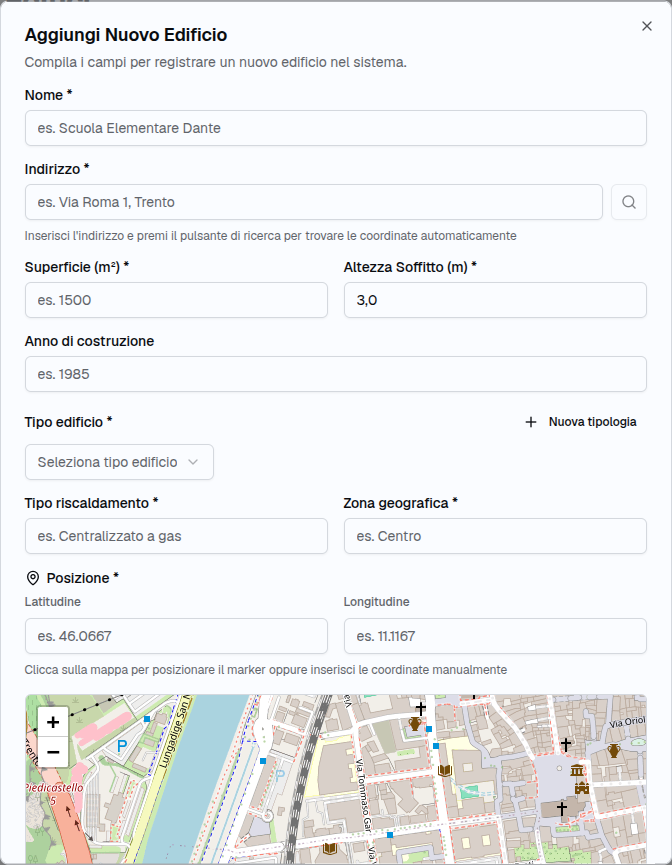
\includegraphics[width=0.5\linewidth]{../images/Frontend/create-building.png}
    \caption{Dialogo per la creazione di un nuovo edificio}
    \label{fig:create-building}
\end{figure}

In \cref{fig:buildings} è presente la sezione dedicata alla visualizzazione di tutti gli edifici.
In alto è presenta una barra di ricerca che permette di ricercare gli edifici per nome, indirizzo, zona geografica, tipologia e stato operativo.
Ogni edificio elencato presenta il nome, l'indirizzo, il numero di sensori attivi e il consumo di corrente dell'edificio.
È inoltre possibile registrare nuovi edifici, come si vede in \cref{fig:create-building}, inserendo i dati anagrafici dell'edifico e la posizione geografica (si accettato sia coordinate che indirizzo).

\subsubsection{Confronto Edifici}
\begin{figure}[H]
    \centering
    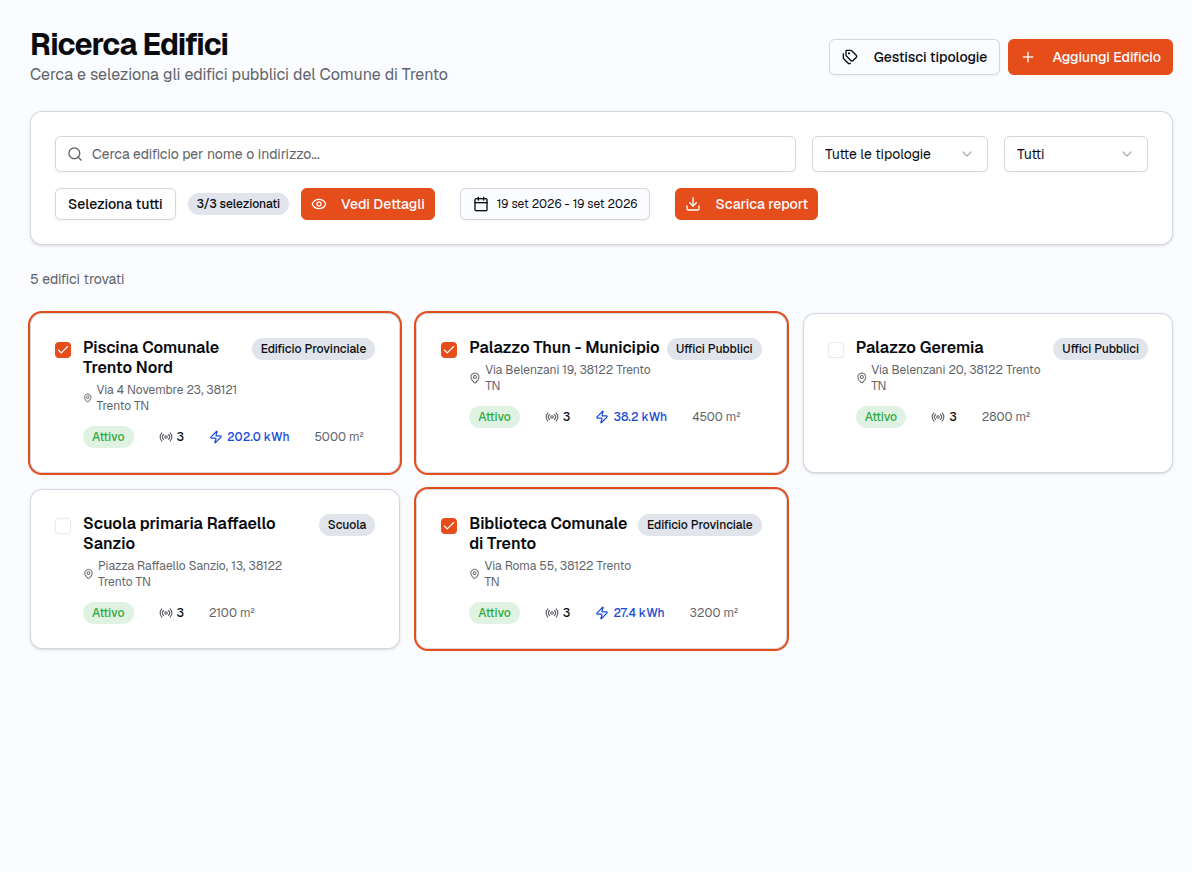
\includegraphics[width=0.8\linewidth]{../images/Frontend/compare-selected.png}
    \caption{Selezione di più edifici}
    \label{fig:building-select}
\end{figure}

\begin{figure}[H]
    \centering
    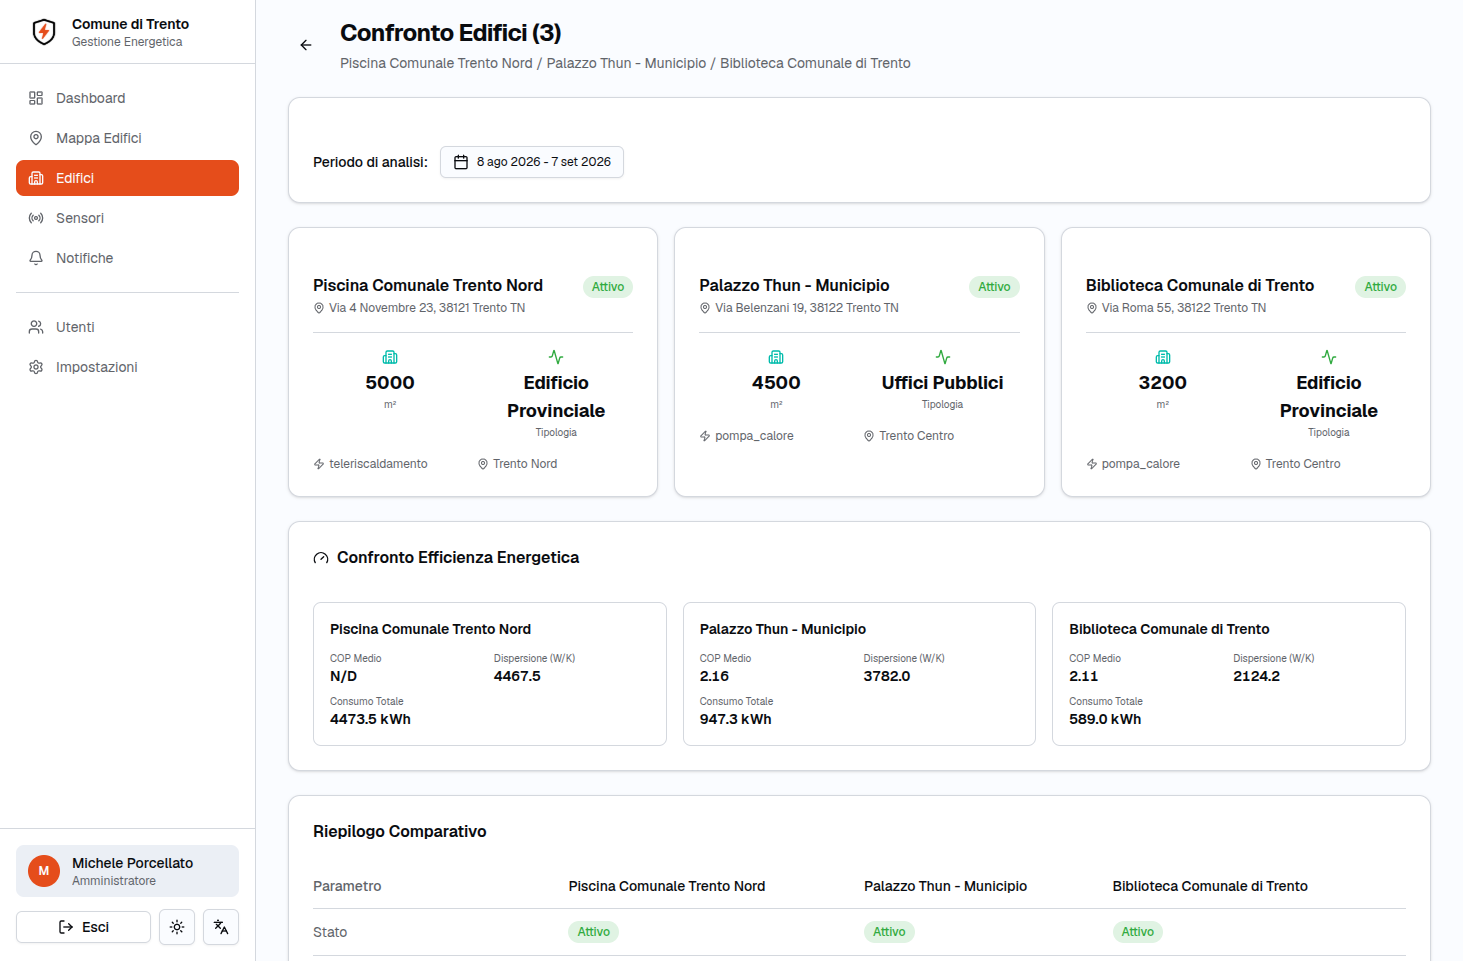
\includegraphics[width=0.8\linewidth]{../images/Frontend/compare-buildings.png}
    \caption{Pagina di comparazione}
    \label{fig:building-compare}
\end{figure}

È possibile confrontare più edifici, selezionandone al massimo 3, come si vede in \cref{fig:building-select}. Da qui è possibile scaricare sia il report dell'efficienza dei vari edifici in PDF che i valori dei vari sensori in CSV.
Cliccando su ``Vedi dettagli'' si apre la visualizzazione comparativa (\cref{fig:building-compare}).
Questa pagina mostra intuitivamente l'efficienza dei vari edifici e lo stato generale degli stessi.

\subsection{Dettaglio edificio}

\begin{figure}[H]
    \centering
    % Prima immagine
    \begin{subfigure}[b]{0.8\textwidth}
        \centering
        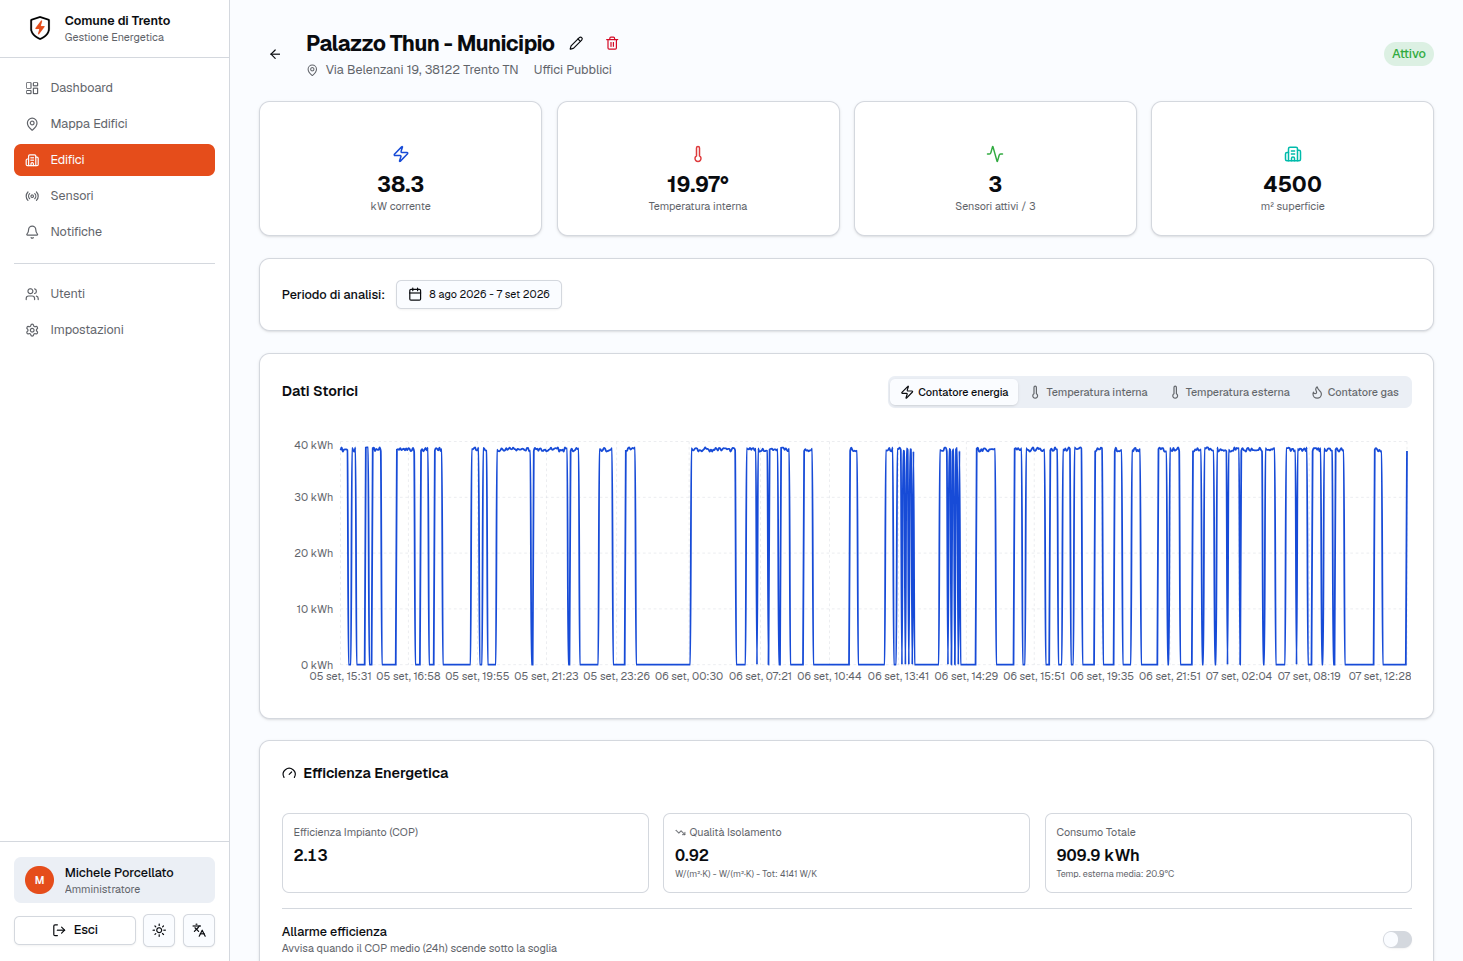
\includegraphics[width=\linewidth]{../images/Frontend/building-example-1.png}
        \label{fig:building-1}
    \end{subfigure}
    \hfill % Spazio orizzontale flessibile per separare le due figure
    % Seconda immagine
    \begin{subfigure}[b]{0.8\textwidth}
        \centering
        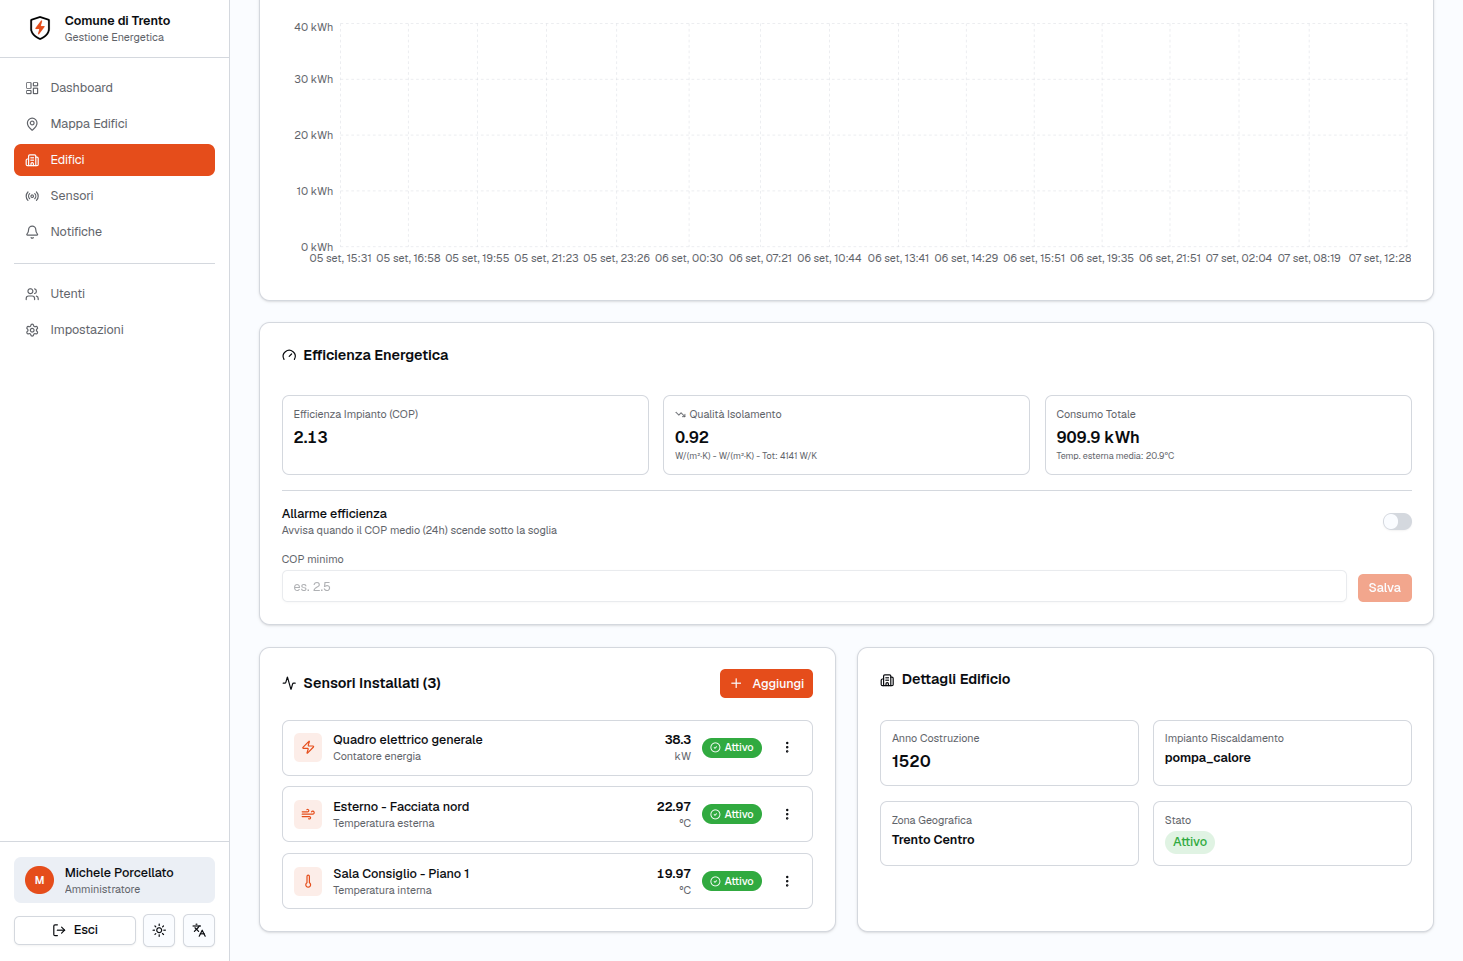
\includegraphics[width=\linewidth]{../images/Frontend/building-example-2.png}
        \label{fig:building-2}
    \end{subfigure}
    
    \caption{Pagina di dettaglio dell'edificio}
    \label{fig:building-detail}
\end{figure}

La pagina di dettaglio di un edificio riunisce i dati anagrafici e di contesto, i valori in tempo reale rilevati dai sensori, quali la temperatura interna, la temperatura esterna e il consumo istantaneo, aggiornati automaticamente, i grafici storici dei consumi e delle temperature con la possibilità di selezionare l'intervallo temporale e la grandezza di interesse, e le metriche di efficienza termica dell'edificio nel periodo selezionato, tra cui l'energia consumata, la temperatura esterna media, la dispersione termica stimata e il coefficiente di prestazione medio.

\subsection{Sensori}

\begin{figure}[H]
    \centering
    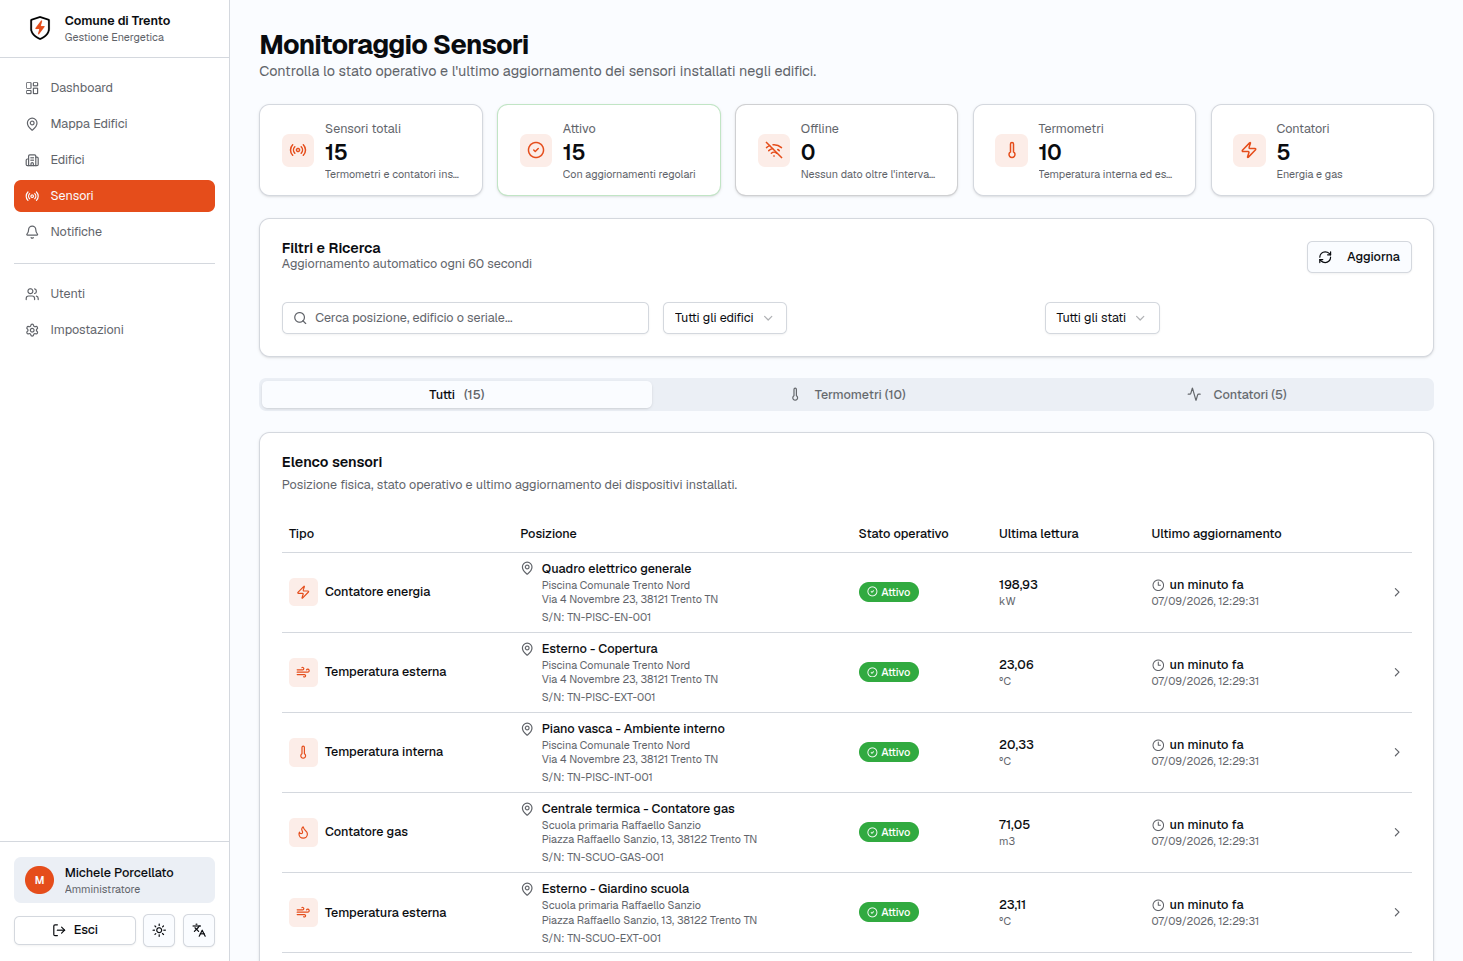
\includegraphics[width=0.8\linewidth]{../images/Frontend/sensors.png}
    \caption{Sezione sensori}
    \label{fig:sensors}
\end{figure}

\begin{figure}[H]
    \centering
    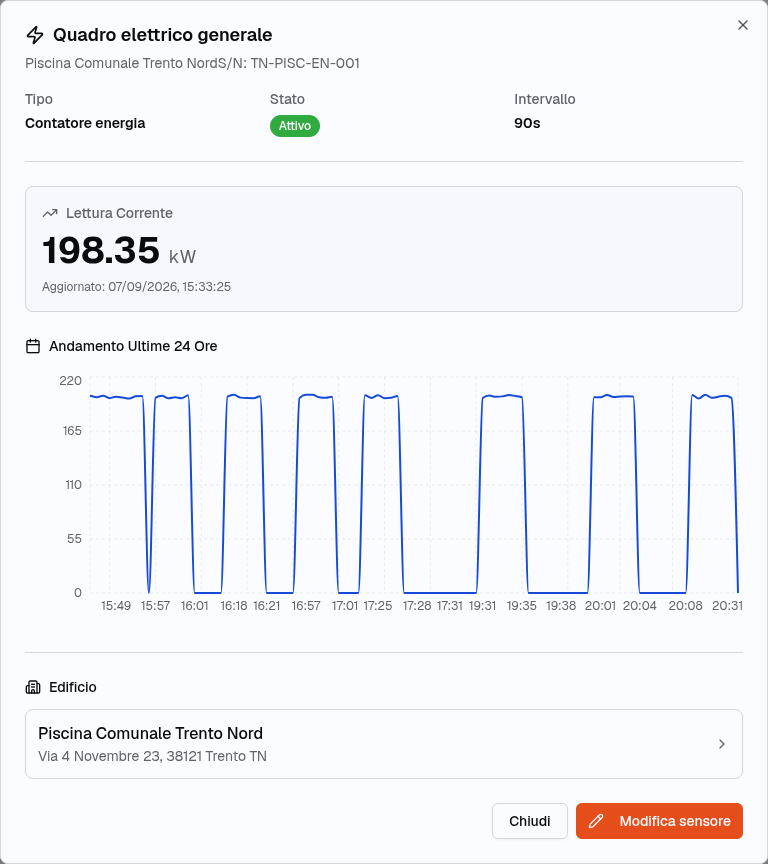
\includegraphics[height=0.5\linewidth]{../images/Frontend/sensors-detail.png}
    \caption{Dettaglio sensore}
    \label{fig:sensors-detail}
\end{figure}

In \cref{fig:sensors} è presente la sezione sensori. Essa comprende la gestione e il monitoraggio dei dispositivi installati. 
La pagina permette di registrare nuovi sensori, eseguire nuove ricerche e filtrarli per tipologia, oltre a vedre il loro stato operativo.
Cliccando sul sensore è possibile vederne i dettagli (\cref{fig:sensors-detail});
Da qui, andando su modifica sensore è possibile configurarne la tipologia, la posizione, l'intervallo di trasmissione e le soglie di allarme minima e massima.

\subsection{Allarmi}

\begin{figure}[H]
    \centering
    % Prima immagine
    \begin{subfigure}[b]{0.50\textwidth}
        \centering
        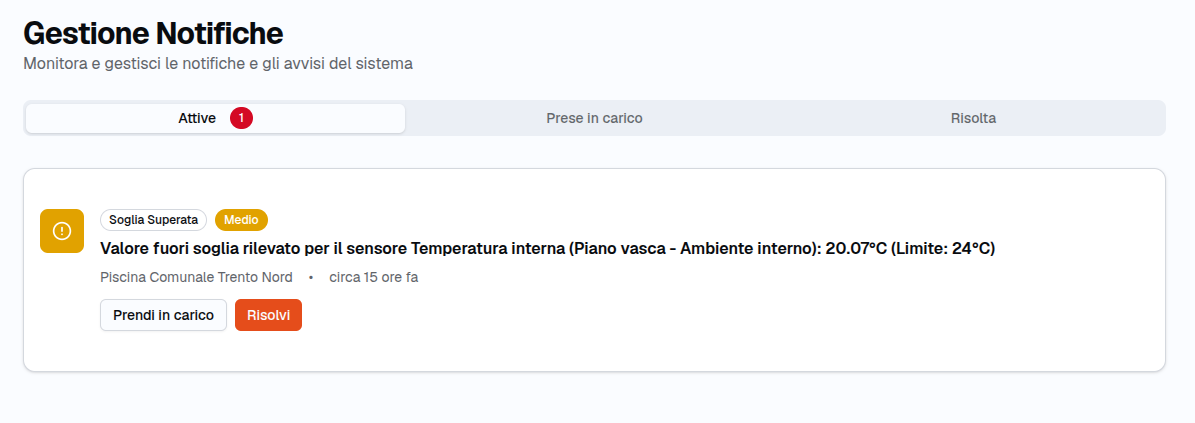
\includegraphics[width=\linewidth]{../images/Frontend/alert3.png}
        \caption{}
        \label{fig:alert-1}
    \end{subfigure}\hfill
    % Seconda immagine
    \begin{subfigure}[b]{0.50\textwidth}
        \centering
        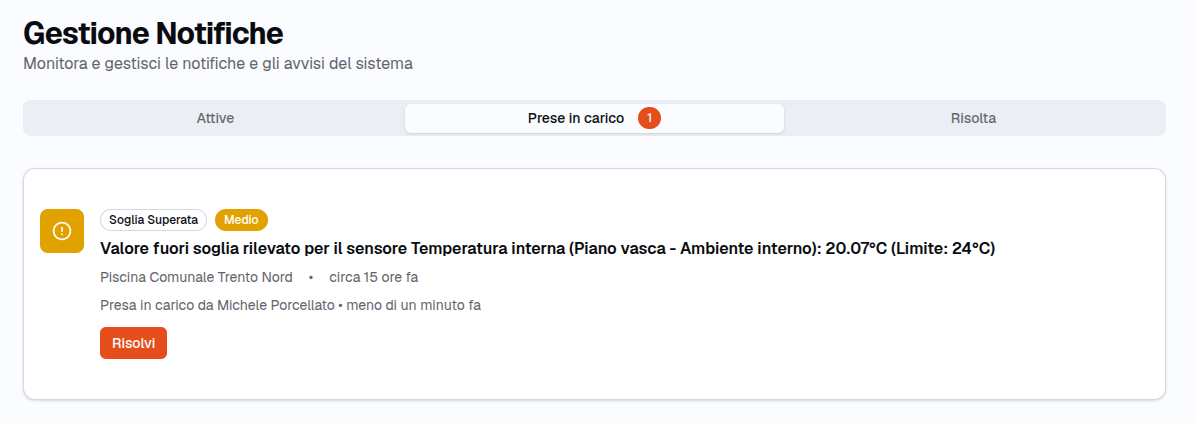
\includegraphics[width=\linewidth]{../images/Frontend/alert2.png}
        \caption{}
        \label{fig:alert-2}
    \end{subfigure}\hfill
    % Terza immagine
    \begin{subfigure}[b]{0.50\textwidth}
        \centering
        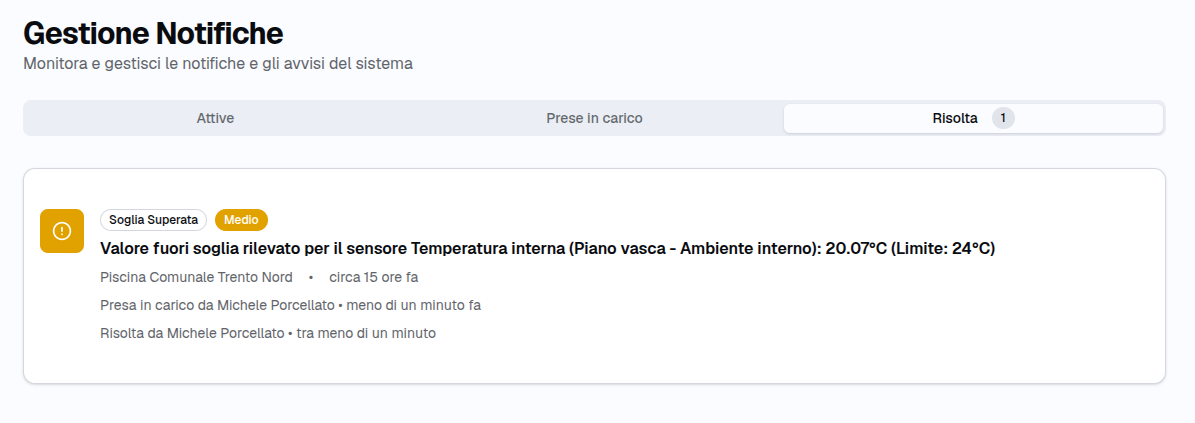
\includegraphics[width=\linewidth]{../images/Frontend/alert1.png}
        \caption{}
        \label{fig:alert-3}
    \end{subfigure}
    
    \caption{Pagina di gestione degli allarmi}
    \label{fig:alert}
\end{figure}

La pagina degli allarmi (\cref{fig:alert}) raggruppa le notifiche generate dal sistema.
Esse sono filtrabili per stato e ordinate di default per timestamp. 
Per ciascun allarme è possibile consultare i dettagli, prenderlo in carico o risolverlo.

\subsection{Amministrazione}
Le sezioni riservate agli amministratori comprendono la gestione degli utenti e le impostazioni di sistema.

\subsubsection{Utenti}
\begin{figure}[H]
    \centering
    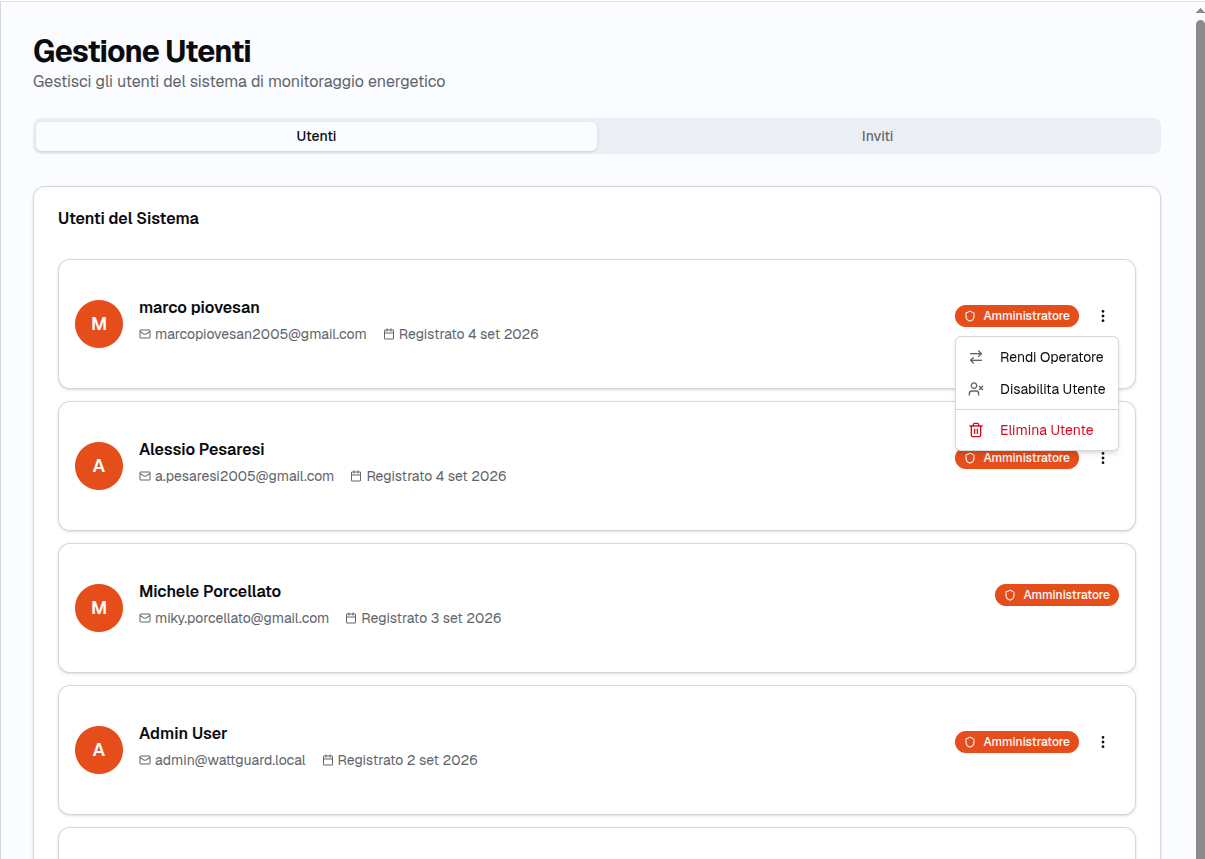
\includegraphics[width=0.8\linewidth]{../images/Frontend/users.png}
    \caption{Sezione utenti}
    \label{fig:users}
\end{figure}

\begin{figure}[H]
    \centering
    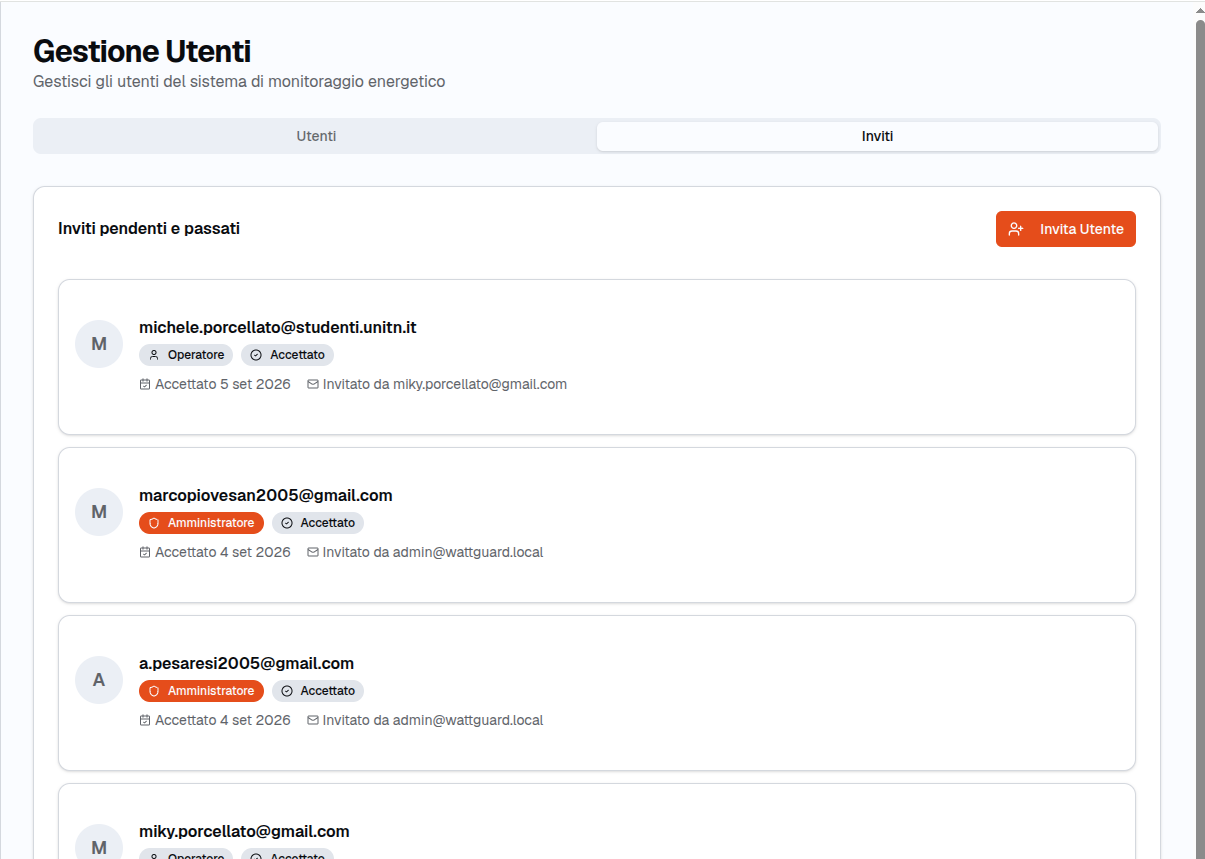
\includegraphics[width=0.8\linewidth]{../images/Frontend/invites.png}
    \caption{Sezione inviti}
    \label{fig:invites}
\end{figure}

\begin{figure}[H]
    \centering
    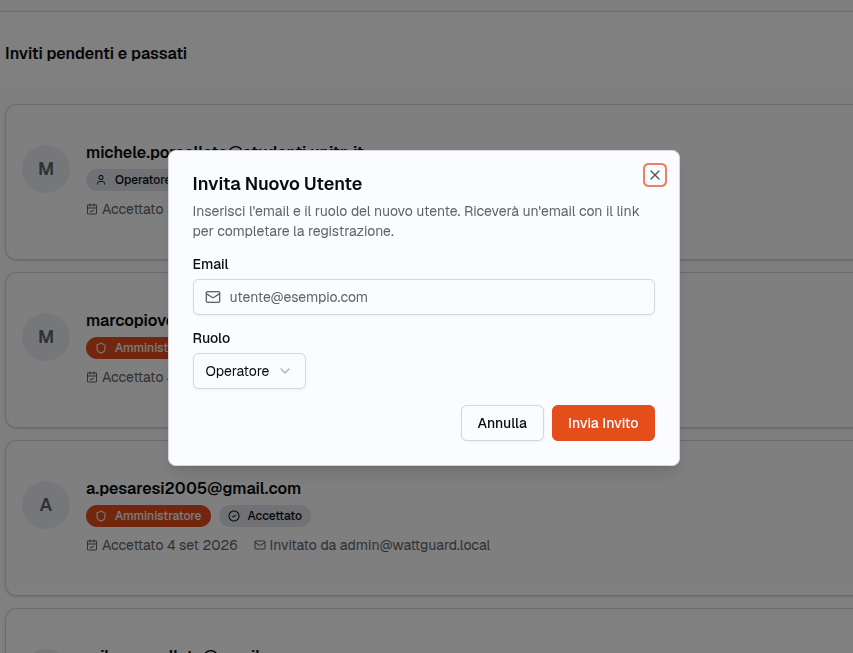
\includegraphics[width=0.5\linewidth]{../images/Frontend/invite-new-user.png}
    \caption{Dialogo invito nuovo utente}
    \label{fig:invites-dialog}
\end{figure}

Nella sezione utenti (\cref{fig:users}) è possibile controllare gli utenti presenti, cambiare il loro ruolo, disattivarli o eliminarli completamente dal sistema.

Per aggiungere nuovi utenti, è necessario recarsi nella sezione inviti (\cref{fig:invites}). Qui sono disponibili gli inviti presenti con lo stato (accettato o in attesa) e la possibilità di aggiungere nuovi utenti al sistema usando la finestra di dialogo mostrata in \cref{fig:invites-dialog}.

\subsubsection{Impostazioni di sistema}
\begin{figure}[H]
    \centering
    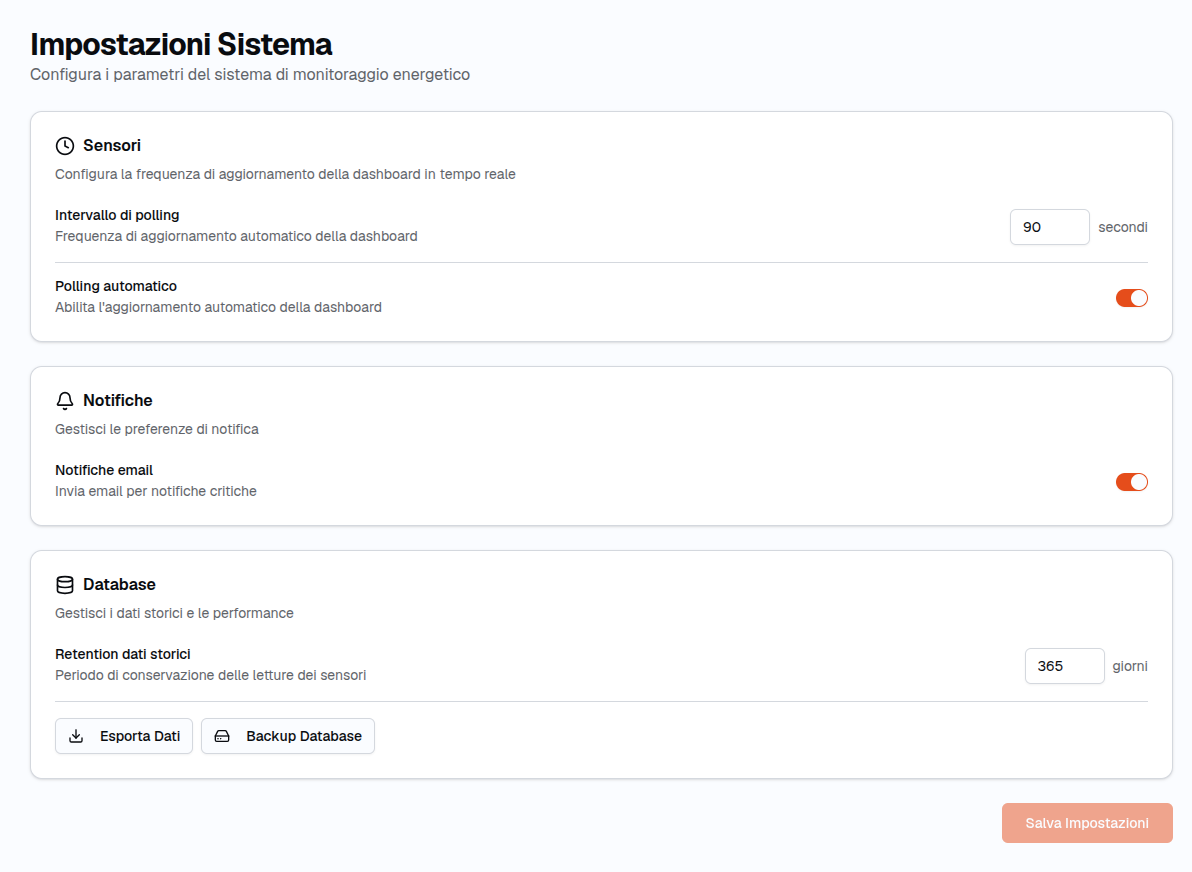
\includegraphics[width=0.8\linewidth]{../images/Frontend/settings.png}
    \caption{Impostazioni di sistema}
    \label{fig:settings}
\end{figure}

Nella pagina di impostazioni di sistema (\cref{fig:settings}) gli amministratori possono configurare l'intervallo di polling per l'aggiornamento dei valori dell'applicazione, gestire se ricevere notifiche email in caso ci siano allerte presenti e gestire i dati storici dell'applicazione (durata di conservazione, esportazione delle letture e backup del database in file JSON)
